\section{相关工作}
\label{sec:related_work}

在本节中,我们回顾了与我们工作最相关的研究方向,\ie,图像检索和视觉位置识别。

\subsection{图像检索}

图像检索是计算机视觉中的一项基础且成熟的任务,其目标是在一个大型数据库中搜索与给定查询图像相似的图像。图像检索过程通常包括两个阶段:全局检索和重排序。在第一个阶段,使用聚合局部特征的全局描述符从大型数据库中检索出 $k$ 个候选图像。随后通过局部特征匹配进行空间验证,以对这 $k$ 个候选图像进行重排序。早期研究依赖于手工设计的特征 \cite{Lowe2004DistinctiveIF, BAY2008346},而当前的方法则利用深度网络学习具有区分力的表示 \cite{cao2020unifyingdeeplocalglobal, radenović2018finetuningcnnimageretrieval}。

大多数图像检索方法关注于选择多样且相关的图像,以帮助用户在真实应用中发现符合其兴趣或需求的选项 \cite{Wan2014DeepLF}。尽管这些方法在检索相似图像方面表现出色,但它们通常缺乏对类别区分或精确 ReID 的重视 \cite{10.1145/1348246.1348248}。与此 \mbox{相比},我们的方法优先考虑实现精确的 ReID。我们遵循“全局检索和重排序”的流程,首先利用全局上下文特征识别排名前五的房间候选项。随后,我们的面向物体的机制以由粗到细的方式细化搜索,逐步区分候选项,直至识别出最相似的房间,从而获得准确的结果。

\begin{figure*}[ht]
    \centering
    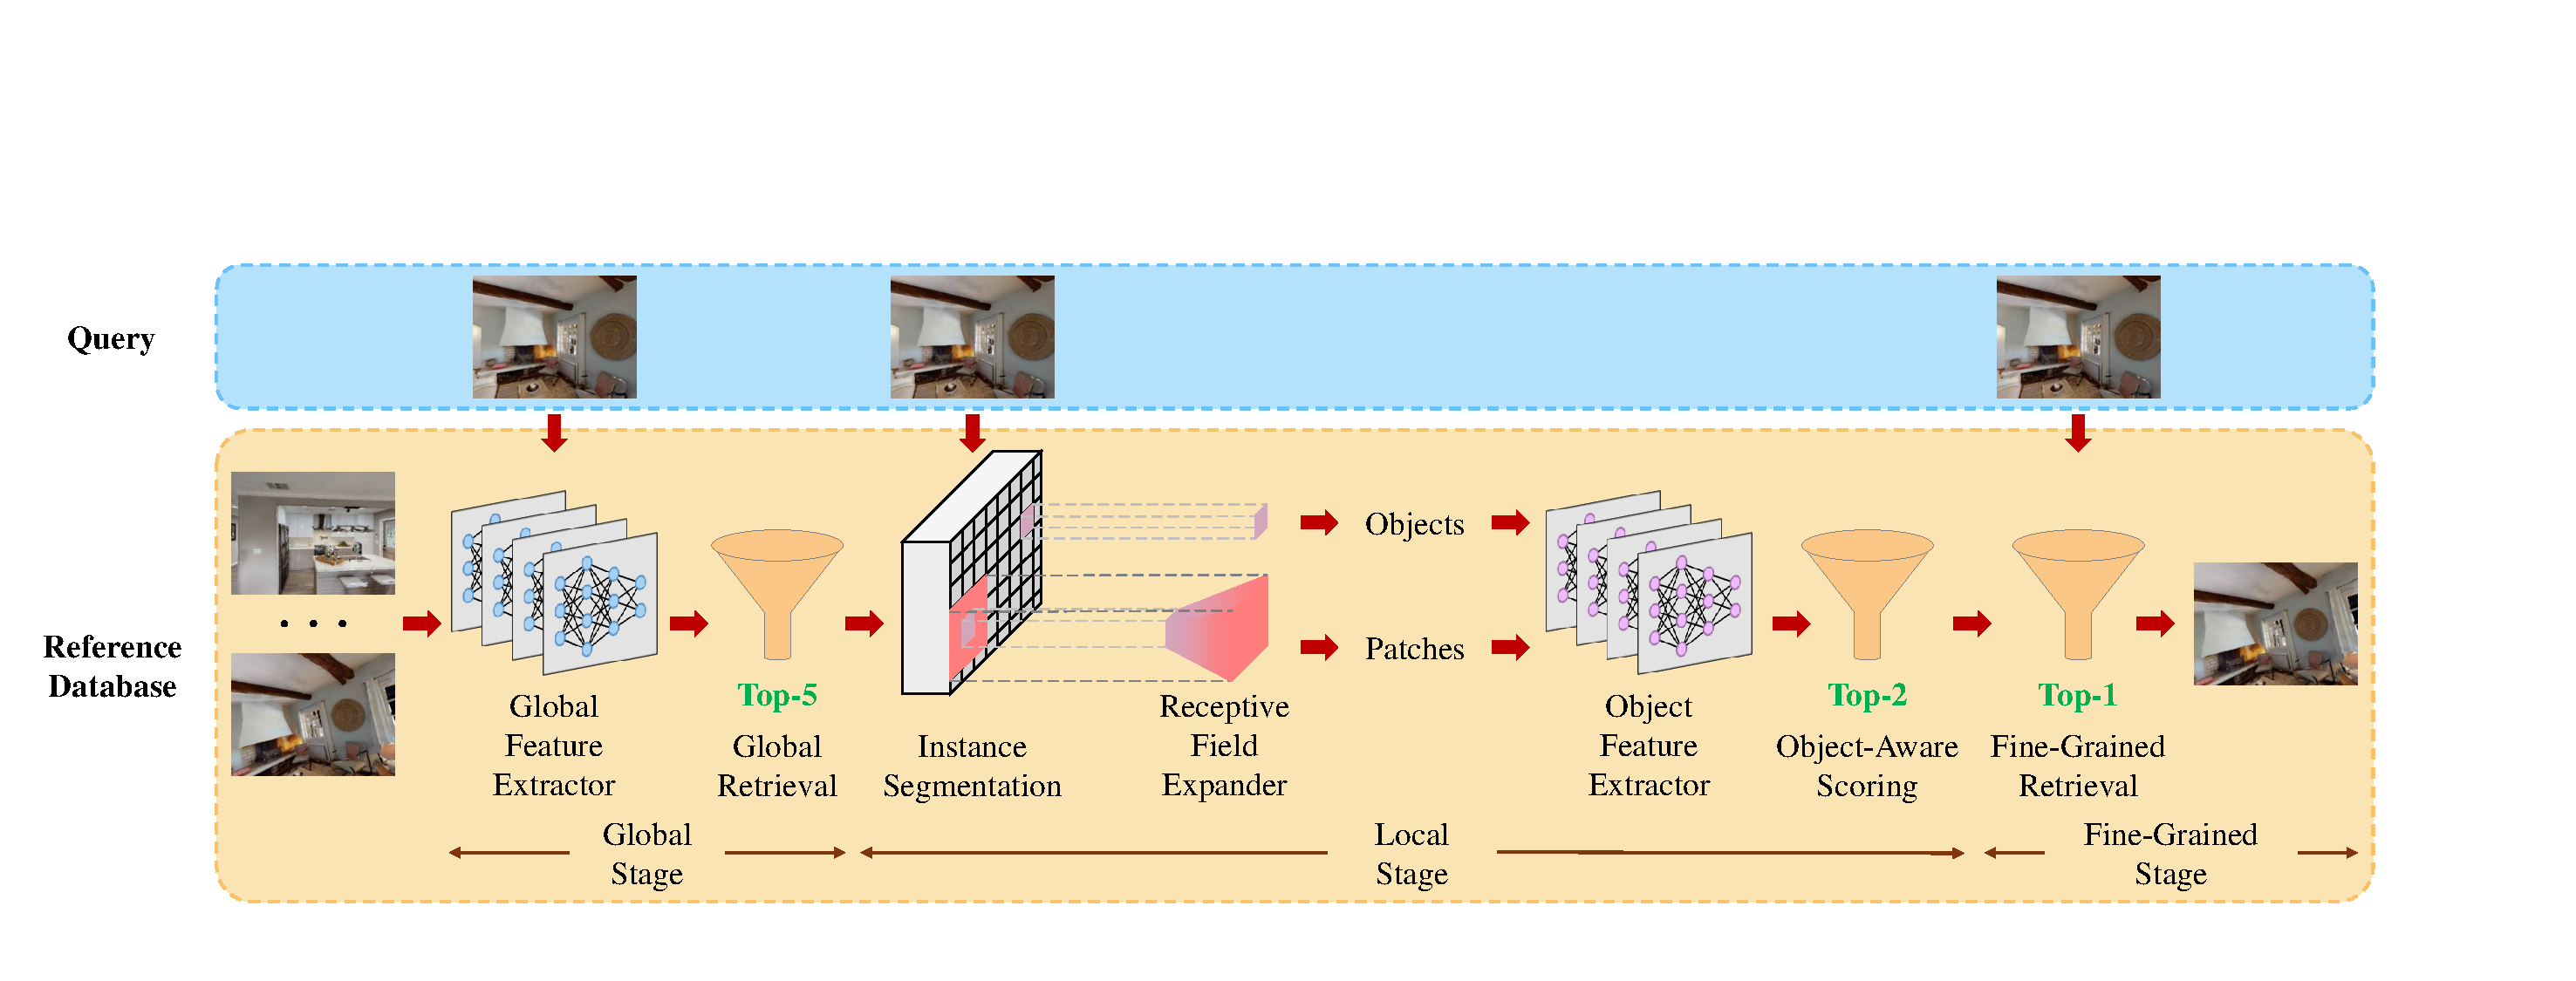
\includegraphics[width=\textwidth]{pipeline_font.pdf}
    \vspace{-16pt}
    \caption{\textbf{AirRoom 粗到细的处理流程}。该流程首先由 Global Feature Extractor 开始,捕获全局上下文特征以检索前 5 张参考图像。然后通过 Instance segmentation 生成目标掩码,接着 Receptive Field Expander 提取目标图像块。Object Feature Extractor 对目标和图像块特征进行处理。Object-Aware Scoring 模块将候选图像缩小到前 2 张,最后 Fine-Grained Retrieval 识别出最合适的参考图像。}
    \vspace{-15pt}
    \label{fig:pipeline}
\end{figure*}
\subsection{视觉位置识别}

视觉位置识别(VPR)通常被框架化为一个特殊的图像检索问题,旨在将某一位置的视图与在不同条件下拍摄的同一地点的图像进行匹配。
先前的方法分为两类:直接使用全局描述符的方法和将局部特征聚合为全局描述符的方法。早期依赖全局描述符的方法主要使用基于卷积神经网络(CNN)的骨干网络,如ResNet \cite{he2015deepresiduallearningimage},来生成这些描述符。然而,最近的方法则利用DINOv2等基础模型 \cite{oquab2024dinov2learningrobustvisual} 来增强特征表示。在聚合类别中,早期技术采用了手工制作的特征,如SIFT \cite{Lowe2004DistinctiveIF}、SURF \cite{10.1007/11744023_32} 和ORB \cite{6126544}。后来的进展,包括NetVLAD系列 \cite{arandjelović2016netvladcnnarchitectureweakly, hausler2021patchnetvladmultiscalefusionlocallyglobal} 和AnyLoc \cite{keetha2023anylocuniversalvisualplace},采用了基于学习的模型来提取特征图,并将局部特征结合成全面的全局描述符。

然而,大多数VPR方法的高性能主要归功于在专门的VPR数据集上进行的大规模训练 \cite{keetha2023anylocuniversalvisualplace}。由于日光、天气和季节的自然变化,收集户外场景的广泛数据相对简单。然而,在室内房间中进行此类数据收集则更加困难,这使得在室内数据集上进行大规模训练变得困难,并可能限制其有效性。
我们的方法通过专注于面向物体的特征表示有效地解决了这一挑战,允许我们利用成熟的预训练模型进行物体特征学习。这一设计使得AirRoom能够在无需对特定数据集进行额外训练或微调的情况下,提供强大的性能。
